\chapter{Embasamento teórico}
No que diz respeito à modelagem molecular, diversas técnicas computacionais podem ser empregadas para o estudo de sistemas microscópicos.
Alguns desses métodos se baseiam na teoria da mecânica quântica para descrever satisfatoriamente o comportamento eletrônico do sistema. 
Uma vez que elétrons são partículas intrinsicamente quânticas, sua descrição correta só é possível com esses métodos.
Como sistemas químicos são governados por processos eletrônicos, técnicas de simulação que levem em conta essa característica quantizada do sistema devem ser utilizados.
Porém, cálculos quânticos são de elevado custo computacional e mesmo com os grandes avanços em eficiência de algoritmos e novos métodos para reduzir esse custo, o estudo de grandes sistemas ainda é um problema nos dias de hoje.

Muitas vezes estamos interessados somente em propriedades físicas (não-eletrônicas) do sistema. Nesses casos, podemos fazer algumas aproximações com o objetivo de simplificar o tratamento teórico.
Uma primeira consideração que pode ser feita é considerar que os átomos como um todo sejam esferas modeladas por um potencial efetivo incluindo de forma média e implícita as propriedades eletrônicas, o que permite a eliminar o cálculo explícito relativo aos graus de liberdade dos elétrons..
A função de energia potencial que descreve o sistema deve ser parametrizada com o auxílio de propriedades experimentais ou de cálculos quânticos de alto nível.
O conjunto de parâmetros e de formas funcionais utilizados para a construção do potencial é chamado de campo de força.
Após parametrizado, o campo de força pode ser utilizado por alguma das técnicas de simulação clássica. Dentre essas técnicas, destacamos a dinâmica molecular clássica\cite{Jensen2017}.

\section{Dinâmica Molecular}

Dinâmica molecular consiste em resolver as equações de movimento da mecânica clássica para um sistema de muitos corpos.
Do ponto de vista do esforço computacional, a dinâmica molecular clássica (onde o hamiltoniano considerado é clássico) é uma técnica sigficativamente menos custosa que os métodos quânticos e, por isso, torna possível o estudo de sistemas maiores.

%ela é uma técnica sigficativamente mais leve que os métodos quânticos e, por isso, se torna possível o estudo de sistemas maiores.

Nesta técnica, é necessário a definição das posições e velocidades iniciais dos átomos constintuintes do sistema.
Com base no campo de força e nas posições atuais, podemos calcular a força atuante em cada um dos átomos do sistema.
Então resolve-se a equação de Newton para calcular sua nova posição em um passo futuro.
O novo conjunto de coordenadas é então utilizado para recalcular as forças e assim pode-se avaliar a evolução temporal do sistema com base na integração numérica das equações de movimento\cite{Frenkel2002}.

Uma vez obtida a trajetória do sistema, pode-se fazer uso da mecânica estatística para calcular as propriedades desejadas do sistema. 

\subsection{O campo de força}

Pode-se descrever a forma funcional do campo de força de diversas formas.
Uma possibilidade, a que foi utilizada neste trabalho, é\cite{Leach2001}:

\begin{equation}
\begin{aligned}
V(r) = &\sum_{b} \frac{k_{b}}{2}(r_{b,eq}-r_{b})^2 \;+\\
       &\sum_{a} \frac{k_{a}}{2}(\theta_{a,eq}-\theta_{a})^2\;+\\
       &\sum_{d} \frac{V_t}{2}(1+cos(n\omega_{d}+\gamma))\;+\\
       &\sum_{i} \frac{V_i}{2}(\xi_{i,eq} - \xi_i)^2\;+\\
       &\sum_{i=1}^N \sum_{j=i+1}^N \left(4\epsilon_{ij}\left[\left(\frac{\sigma_{ij}}{r_{ij}}\right)^{12} - \left(\frac{\sigma_{ij}}{r_{ij}}\right)^{6}\right] + \frac{q_i q_j}{4\pi \epsilon_0 r_{ij}} \right)
\end{aligned}
\label{FF}
\end{equation}

onde $k_{b}$, $r_{b,eq}$, $k_{a}$, $\theta_{a,eq}$, $V_t$, $n$, $\gamma$ e $\xi_{i,eq}$ são parâmetros dos potenciais ligados; $\epsilon_{ij}$, $\sigma_{ij}$, $q_i$, $q_j$ são parâmetros dos potenciais não ligados e devem ser ajustados empiricamente.
A variáveis $r_{b}$, $r_{ij}$, $\theta_{a}$, $\omega_{d}$ e $\xi_{i}$ são a distância entre dois átomos ligados e não ligados, o ângulo formado por três átomos ligados em série, o ângulo formado pelo torsional de diedro próprio e o impróprio, respectivamente.
Os termos da Equação \ref{FF} são referentes aos graus de liberdade ilustrados na Figura \ref{CampoDeForca}.

\begin{figure}[ht!]
\centering
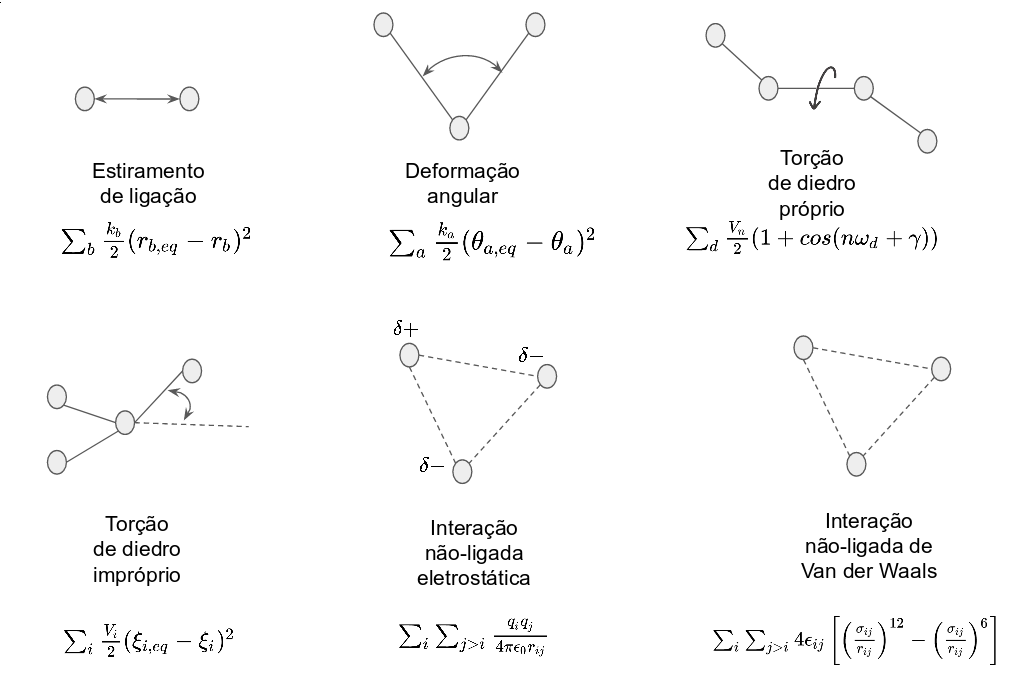
\includegraphics[width=0.9\textwidth]{CampoDeForca.png}
\caption{Representação esquemática das deformações responsáveis pela energia potencial no sistema. Pela ordem de aparecimento dos termos na Equação \ref{FF}, estiramento de ligação, estiramento angular, estiramento de diedro e interações não-ligadas.}
\label{CampoDeForca}
\end{figure}

A forma como os átomos são tratados no campo de força também pode ser diferente entre cada modelo.
A forma mais completa é conhecida como uma abordagem \textit{all-atoms} e consiste em incluir, explicitamente, todos os átomos do sistema nos seus cálculos.
A fim de possibilitar a simulação de sistemas ainda maiores, alguns átomos podem ser tratados em conjunto como um pseudo-átomo.
Essa abordagem é conhecida como \textit{united-atoms} ou \textit{coarse grained}, dependendo de quantos átomos são omitidos do seu modelo\cite{Allen2017}.
Como discutido anteriormente, o 2016H66\cite{Horta2016} é um modelo \textit{united-atoms}, ou seja, seus átomos de hidrogênio apolares são tratados em conjunto com os átomos de carbonos aos quais estão ligados.
Dessa forma, os grupos CH$_n$ são tratados como um único pseudo-átomo.

A definição da forma funcional, o valor dos parâmetros propriamente ditos, assim como outros parâmetros utilizados na simulação (como o raio de corte $r_c$ do modelo, por exemplo, que veremos mais a frente) compõem o campo de força.
É importante ressaltar que o conjunto de condições utilizadas na parametrização é de significativa importância para a reprodutibilidade dos resultados obtidos com os campos de força disponíveis na literatura.
Como mostrado em um estudo sistemático por Gonçalvez \textit{et al}\cite{Goncalvez2018}, uma mudança arbitrária das condições de simulação podem causar mudanças substanciais nos resultados obtidos.

\subsection{Integração das equações de movimento}

A princípio, as funções que regem as equações de movimento são contínuas. Para que possamos integrá-las numéricamente precisamos discretizar o tempo e utilizar um algoritmo de integração.
Dentre os algoritmos conhecidos, alguns poucos se tornaram populares para uso em dinâmica molecular por atenderem os requisitos de conservação de energia, reversibilidade temporal e por serem bem escaláveis quanto ao custo computacional\cite{Frenkel2002}.
O algoritmo utilizado nesse trabalho foi o \textit{leap-frog}, que usa as seguintes relações para a evolução temporal da posição e da velocidade\cite{Leach2001}:

\begin{equation}
\begin{aligned}
& \textbf{r}(t+\delta t)=\textbf{r}(t)+\delta t \times \textbf{v}(t+\frac{1}{2}\delta t)\\
& \textbf{v}(t+\frac{1}{2}\delta t)=\textbf{v}(t-\frac{1}{2}\delta t)+\delta t \frac{\textbf{F}(t)}{m}
\end{aligned}
\label{leap-frog}
\end{equation}
onde $\textbf{r}$ e $\textbf{v}$ são os vetores de coordenadas e velocidade, respectivamente, $\delta t$ é o incremento no tempo (ou passo de tempo), $\textbf{F}$ é a força resultante na partícula e $m$ a sua massa.

O \textit{leap-frog} tem a vantagem, em relação ao algoritmo de Verlet (um dos mais utilizados em simulações de dinâmica molecular), de incluir a velocidade explicitamente no seu equacionamento, dessa forma a velocidade é mais consistentemente calculada.
Uma desvantagem, é que o conjunto de coordenadas e de velocidades não são avaliados no mesmo instante de tempo. 
Como pode ser visto nas relações mostradas na Equação \ref{leap-frog}, a integração é feita primeiro na velocidade, calculando o seu valor em um tempo de $\frac{1}{2}\delta t$ futuro. E então esse valor de velocidade é utilizado para calcular as coordenadas em $\delta t$.
Portanto, estimativas sobre o valor total de energia (soma da cinética e potencial) não podem ser avaliadas diretamente com o uso desse algoritmo.
Contudo, ele já foi altamente validado em trabalhos da área e, como as propriedades de interesse (Ver \ref{Propriedades}) dependem unicamente das posições, essa desvantagem não será um problema para este estudo\cite{Leach2001}.

A simples integração das equações de movimento não possibilita o controle das condições de simulação (principalmente temperatura e pressão).
De fato, é possível mostrar que uma simulação desse tipo mantém o número de partículas, o volume do sistema e a energia contantes.
Ou seja, o conjunto estatístico, ou o \textit{ensemble}, natural é o micro-canônico\cite{Tuckerman2010}.
Como os experimentos são, geralmente, realizados à temperatura e pressão constantes, as equações de movimento são, geralmente, modificadas para fornecer o ensemble isotérmico-isobárico.
Isso é feito adicionando termos extras no hamiltoniano que levem em conta um banho externo para controle da pressão e da temperatura.

\subsection{Outros ensembles}

Da mecanica estatística, sabe-se que o valor médio da energia no ensemble canônico é proporcional à termeratura\cite{Leach2001}.
De fato:

\begin{equation}
{\left< {H} \right>}_{NVT} = \frac{3}{2}Nk_bT ,
\end{equation}
onde $H$ é o Hamiltoniano, $N$ é o número de partículas, $k_b$ a constante universal de Boltzmann e $T$ a temperatura.

Na ausência de campo externo, o Hamiltoniano de um gás ideal é dado pela soma as energias cinéticas de todas as partículas do sistema.
De forma que podemos isolar a temperatura da seguinte forma:

\begin{equation}
T=\frac{1}{2} \sum_{i=1}^{N} {\frac{2}{3}\frac{m_i v_i^2}{Nk_b}}
\end{equation}
onde $m_i$ e $v_i$ são,respectivamente, a massa e a velocidade da partícula $i$ no somatório.

A primeira forma utilizada para controle da temperatura foi idealizada por Woodcock\cite{Woodcock1971} em 1971 e consiste em multiplicar as novas velocidades por um fator de escala para forçar o sistema a manter a mesma temperatura.
Isto é, ele propôs que a variação de temperatura fosse escrita da seguinte forma:

\begin{equation}
\Delta T = T_{new} - T_{curr}=\frac{1}{2} \sum_{i=1}^{N} {\frac{2}{3}\frac{m_i (\lambda v_i)^2}{Nk_b}} - \frac{1}{2} \sum_{i=1}^{N} {\frac{2}{3}\frac{m_i v_i^2}{Nk_b}}
\end{equation}
onde $T_{new}$ é a temperatura no passo de integração seguinte, $T_{curr}$ a temperatura no atual passo e $\lambda$ é o fator de escala.

Que pode ser reescrito como:

\begin{equation}
\begin{aligned}
&\Delta T = (\lambda ^2 - 1) T_{curr}\\
&\text{com} \; \lambda =  \sqrt{\frac{T_{new}}{T_{curr}}}
\end{aligned}
\end{equation}

Dessa forma, ao selecionar $T_{new}$ fazemos com que o sistema corrija as velocidades de forma a manter $T_{curr}$ em torno de um valor próximo de $T_{new}$.

Outra forma mais utilizada hoje em dia é controlar a temperatura com base no acoplamento com um banho externo mantido à temperatura constante.
Esse método é uma generalização do metódo de Woodcock\cite{Woodcock1971}.
Ele foi desenvolvido por Berendsen\cite{Berendsen1984} em 1984 e é largamente utilizado até hoje.
Nele, associamos a variação da temperatura com a diferença entre o banho externo e o sistema:

\begin{equation}
\frac{dT(t)}{dt} = \frac{1}{\tau}\left( T_{bath}-T(t) \right)
\end{equation}
onde $\tau$ é uma constante de acoplamento que determina o quão fortemente acoplado os sistemas estão, $T_{bath}$ é a temperatura do banho externo e $T(t)$ é a temperatura no sistema simulado.

Esse método dá uma variação exponencial na temperatura do sistema até a convergência para a temperatura do banho.
A cada passo, a temperatura é atualizada de:

\begin{equation}
\Delta T = \frac{\delta t}{\tau}\left( T_{bath}-T(t) \right)
\end{equation}

Essa variação fornece um fator de escala $\lambda$ com a forma:

\begin{equation}
\lambda ^2 = 1 + \frac{\delta t}{\tau}\left( \frac{T_{bath}}{T(t)} - 1 \right)
\end{equation}

Dependendo do valor de $\tau$, o acoplamento pode ser fraco e demorar muito para estabilizar a temperatura do sistema, ou forte e inserir ruidos na variação da temperatura.

Uma abordagem semelhante pode ser feita para a pressão, supondo um ``reservatório de volume'' externo que troca volume com o sistema a fim de mantê-lo ao redor de uma pressão definida.
Seguindo o formalismo de Berendsen mostrado anteriormente, é possível chegar em expressões análogas para a pressão que são conhecidos como o barostato de Berendsen, assim como as equações para a temperatura são conhecidas como o termostato de Berendsen.
Extensões, melhorias e outros modelos de acoplamento foram propostos na literatura e são igualmente utilizados atualmente.
Mas como a ideia base da maioria das abordagens é a exibida aqui, não descreveremos cada um dos modelos existentes\cite{Leach2001}.

\subsection{Avaliação da Força}

Sistemas macroscópicos, em geral, possuem um número enorme de moléculas (da ordem de um mol de moléculas).
Isto é, para simular um sistema com apenas um sexto de mol de qualquer substância, seria necessário computar a força entre, aproximadamente, $10^{23}$ moléculas.
Mesmo que o tempo gasto por um computador para efetuar as contas seja muito rápido, a grande quantidade de átomos inviabiliza o cálculo de um sistema dessa escala de tamanho.
Por outro lado, caso o sistema fosse reduzido à uma caixa com alguns poucos átomos, os efeitos do confinamento da substância acarretaria erros nos cálculos das propriedades do sistema de macroscópico de interesse.
Para conseguir simular um sistema de larga escala sem os efeitos de parede causada pela introdução artificial de uma caixa de simulação, é adotada a condição de contorno periódica.
O que é feito, como ilustrado na Figura \ref{RC}, é considerar cópias do sistema simulado em todas as direções.
Dessa forma, somente o sistema central é simulado e as as cópias têm o mesmo comportamento.
De fato, existe a introdução de uma periodicidade inexistente em sistemas reais, mas isso pode ser contornado considerando uma caixa grande o suficiente para que a influência dessa periodicidade artificial possa ser desprezada.

É necessário calcular a força atuante em cada átomo para resolver a equação de movimento para eles.
Pelo princípio da superposição, força em cada um dos átomos é avaliada como uma soma da contribuição de cada interação atuante no mesmo.
Como o campo de força é escrito em termos da energia potencial, as forças podem ser obtidas por: 

\begin{equation}
F=-\nabla V
\end{equation}

Formalmente, os somatórios correm sobre todos os átomos presentes na simulação.
Mas como visto anteriormente, a representação periódica leva a um sistema com infinitos átomos.
Logo, seria impossível avaliar os somatórios sobre todos os átomos.
Contudo, átomos mais distantes praticamente não contribuem dada sua fraca interação devido sua grande distância em relação ao átomo de referência.
É sabido que a avaliação da força é uma das etapas mais lentas nos cálculos de dinâmica molecular, em especial dos termos não-ligados, por isso é evitado calcular a interação entre átomos muito distantes por ela ser praticamente nula.
A fim de agilizar essa etapa, comumente é utilizado um raio de corte $r_c$ como uma distância máxima em que as interações são consideradas\cite{Frenkel2002}, como ilustrado na Figura \ref{RC}.

\begin{figure}[ht!]
\centering
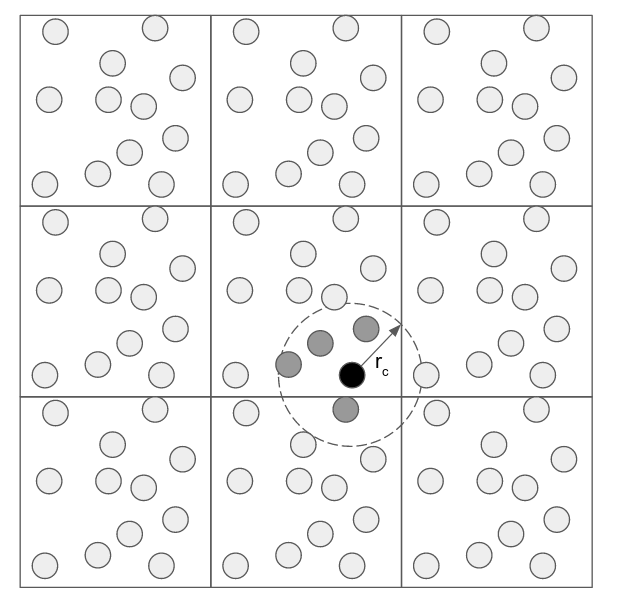
\includegraphics[width=0.5\textwidth]{rc.png}
\caption{Ilustração das condições de contorno periódicas e a consideração de um raio de corte. 
O átomo em preto é o átomo sobre o qual a força está sendo calculada.
O raio de corte é ilustrado por meio do círculo pontilhado.
Os átomos em cinza, dentro do círculho, são os considerados para o cálculo da força no átomo central.}
\label{RC}
\end{figure}

Devido à forma funcional dos potenciais, conforme indicado pela Figura \ref{LJCOUL}, o potencial de Lennard-Jones converge mais rapidamente para zero do que o de Coulomb.
Dessa forma, pode-se definir um raio de corte que contenha todas as interações não-nulas de Lennard-Jones mas que ignore uma parte relevante das interações eletrostáticas.
Um problema de se considerar raio de corte muito grandes é que, dependendo do tamanho da caixa, um átomo pode interagir com sua própria réplica criada pela adoção de condições de contorno periódicas.
A fim de evitar essa artificialidade no sistema, foi popularizada a adoção da convenção de imagem mínima.
Nessa convenção, o raio de corte deve ser, no máximo, metade do tamanho da menor dimensão da caixa de simulação.
Dessa forma, as interações consideradas serão sempre com a réplica do átomo que está mais próximo do átomo central.
Na Figura \ref{RC}, o átomo em preto interage com um átomo em cinza que está é uma replica criada pela inserção da periodicidade. 
Ele não interage com a imagem do átomo em cinza que está dentro da sua própria caixa\cite{Frenkel2002}.

\begin{figure}[ht!]
\centering
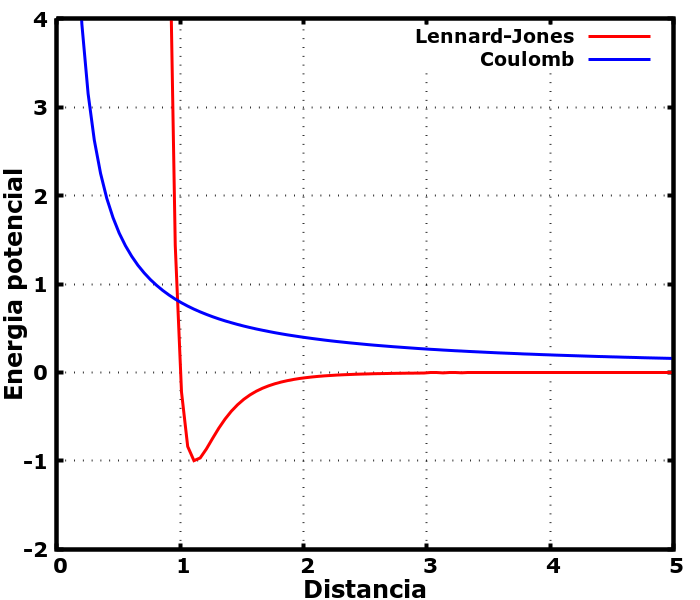
\includegraphics[width=\textwidth]{poten.png}
\caption{Curvas do potencial de Lennard-Jonnes e Coulombiano. As propriedades estão em unidades arbitrárias. Os parâmetros (ver Equação \ref{FF}) $\epsilon, \sigma, q_i \; \text{e} \; q_j$ foram definidos como a unidade e o $\epsilon_0$ como 0.1.}
\label{LJCOUL}
\end{figure}

Para que a força não seja avaliada de forma errada, já que não é possível considerar um raio de corte pequeno devido à forma do potencial eletrostático e nem um grande por causa da convenção de imagem mínima, algumas estratégias são descritas na literatura para contornar esse problema.
As interações de Lennard-Jones podem ser avaliadas com um raio de corte como descrito anteriormente.
Mas as interações eletrostáticas são de longo alcance, e devem ser calculadas com um algoritmo próprio para esse tipo de interação.
Aqui mostraremos uma das metodologias conhecida como \textit{Particle-Mesh-Ewald} (PME)\cite{Darden1993, Essmann1995}.
Nesse método, o somatório das interações eletrostáticas é resolvido para todas as réplicas geradas, para isso, mais um somatório é inserido varrendo todas as caixas de simulação existentes:

\begin{equation}
\begin{aligned}
V = \sum_n \sum_{i}^N \sum_{j>i}^N \frac{q_i q_j}{4\pi \epsilon_0} \frac{1}{r_{ij} + \mathbf{n}}
\end{aligned}
\end{equation}
onde $\mathbf{n}=L_x n_x + L_y n_y + L_z n_z$ é um vetor que varre todas as réplicas de caixas de simulação, $L_i$ é o comprimento da caixa de simulação no eixo $i$.

Esse somatório é de convergência condicional e, quando converge, lenta. 
A adoção de um raio de corte á ineficaz por motivos já discutidos anteriormente. 
A fim de efetuar a soma, essa série é dividida em duas  através da identidade\cite{Leach2001}:

\begin{equation}
\begin{aligned}
\frac{1}{r} = \frac{f(r)}{r} + \frac{1-f(r)}{r}
\end{aligned}
\end{equation}
de tal forma que a função $f(r)$ é escolhida para que as duas novas séries tenham uma boa convergência.

É reportado na literatura que uma boa escolha é a função erro complementar: $f(r) = erfc(\beta |r+n|)$.
Assim, pode-se resolver o primeiro termo no espaço real e o segundo em uma malha no espaço recíproco, onde $\beta$ controla quanto da interação será resolvida em cada um dos espaços.
Na prática, ele é um parâmetro ajustado para otimização de esforço computacional.
Dessa forma, a expressão de fato resolvida são duas séries de rápida convergência\cite{Darden1993, Essmann1995}:

\begin{equation}
\begin{aligned}
V = \sum_n \sum_{i}^N \sum_{j>i}^N \frac{q_i q_j}{4\pi \epsilon_0} \frac{erfc(\beta |r_{ij}+\mathbf{n}|)}{|r_{ij} + \mathbf{n}|} + \frac{1}{\pi V} \sum_{m \neq 0} \frac{exp(-\pi^2 \mathbf{m}^2/\beta)}{\mathbf{m}^2}exp(2\pi i \mathbf{m} * \mathbf{r})
\end{aligned}
\end{equation}
onde $\mathbf{m}$ é o vetor que varre o somatório em todas as réplicas no espaço recíproco e $V$ é o volume da caixa de simulação.

\section{PyPolyBuilder}\label{PyPolyBuilder}
O PyPolyBuilder é um software que está sendo desenvolvido no nosso grupo com o objetivo de facilitar a criação de topologia e coordenadas iniciais de moléculas poliméricas, em especial dendrímeros, para simulação por dinâmica molecular.
Como o aumento do número de átomos cresce exponencialmente com o aumento da geração dos dendrímeros, rapidamente a geração de um arquivo de topologia manualmente se torna inviável (Ver Tabela \ref{tab:pypolybuilder}).
Por isso, é justificada a criação de um software que automatize esse processo.
Aliado à isso, foi feita uma generalização para a criação de estruturas poliméricas em geral.
O software funciona baseado em dois módulos.
O módulo \textit{dendrimer} que é otimizado para a geração de dendrímeros e torna o processo muito mais fácil e o módulo \textit{general} que é generalizado e possibilita a criação de qualquer estrutura polimérica dependendo somente da criatividade do usuário.
Ele se baseia em pequenos blocos de construção que se repetem ao longo da estrutura da molécula desejada e os replica um determinado numero de vezes pedido pelo usuário.
Buscando simplificar o seu uso, um pequeno número de variáveis devem ser definidas pelo usuário na chamada do programa, são elas:
($i$) Nomes dos arquivos dos blocos de construção;
($ii$) arquivo com parâmetros do campo de força;
($iii$) o nome dos arquivos de saída é opcional, mas pode ser definido e
($iv$) o número da geração do dendrímero desejado (no caso do módulo \textit{dendrimer}) ou o arquivo com as ligações entre os blocos (no caso do módulo \textit{general}).

\begin{table}[ht!]
\centering
\caption{Tabela mostrando o aumento do número de átomos com o aumento da geração para dendrímeros PAMAM e PPI em meio com alto pH.}
\begin{tabular}{cc|cc}
\hline
\multicolumn{2}{c|}{PAMAM}   & \multicolumn{2}{c}{PPI} \\
\hline
G & \#Átomos& G & \#Átomos \\
\hline
0 & 48      & 1 &   30\\
1 & 128     & 2 &   70\\
2 & 288     & 3 &   150\\
3 & 608     & 4 &   310\\
4 & 1248    & 5 &   630\\
5 & 2528    & 6 &   1270\\
\hline
\end{tabular}
\label{tab:pypolybuilder}
\end{table}

Como ele é desendolvido em python, o PyPolyBuilder pode ser facilmente utilizado em qualquer computador.
Devido à algumas dificuldades na geração de coordenadas iniciais para o módulo \textit{general} e pela falta de uma validação sistemática até a presente data, o código ainda não foi publicado.


\subsection{Módulo \textit{Dendrimer}}

\begin{figure}[ht!]
\centering
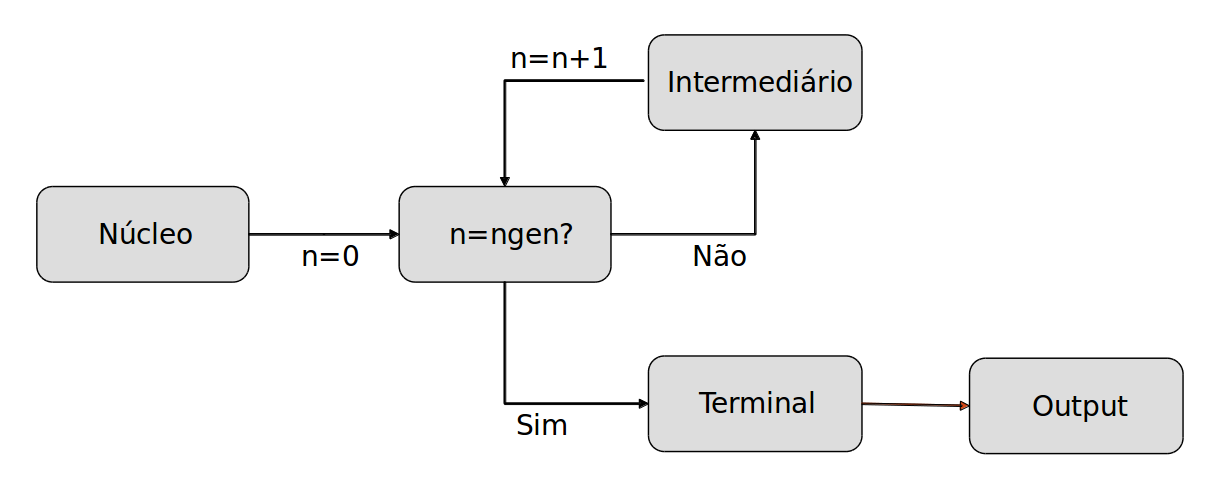
\includegraphics[width=\textwidth]{PyPolyBuilderDend}
\caption{Fluxograma ilustrativo do funcionamento do módulo \textit{dendrimer} do PyPolyBuilder.
O \textit{software} parte do bloco nuclear e compara a geração do dendrímero com a geração pedida pelo usuário. 
Enquanto ele não alcançar o número de geração pedido, uma nova camada de blocos intermediários é conectada.
Quando o tamanho desejado é obtido, uma camada de blocos terminais é conectado e os arquivos de saída são gerados.}
\label{fig:PyPolyBuilderDend}
\end{figure}

O módulo especializado para a geração de dendrímeros usa a simetria da molécula para automatizar a ligação entre os blocos de construção.
Nesse módulo, o usuário precisa fornecer a topologia dos blocos de construção do núcleo, intermediário e terminal, o arquivo de parâmetros do campo de força e o número de geração desejado.
Assim, o PyPolyBuilder parte do núcleo e conecta blocos terminais, camada por camada, até que a geração alcance o valor desejado.
Então os blocos terminais são conectados e a geometria tri-dimensional é gerada seguindo algumas heurísticas.
O usuário pode pedir para uma otimização de geometria ser feita.
Os arquivos de saída (topologia e coordenadas) são escritos em um formato compatível com o software Gromacs\cite{VanDerSpoel2005}.
O fluxograma do programa é exibido na Figura \ref{fig:PyPolyBuilderDend}.


\subsection{Módulo \textit{General}}

\begin{figure}[ht!]
\centering
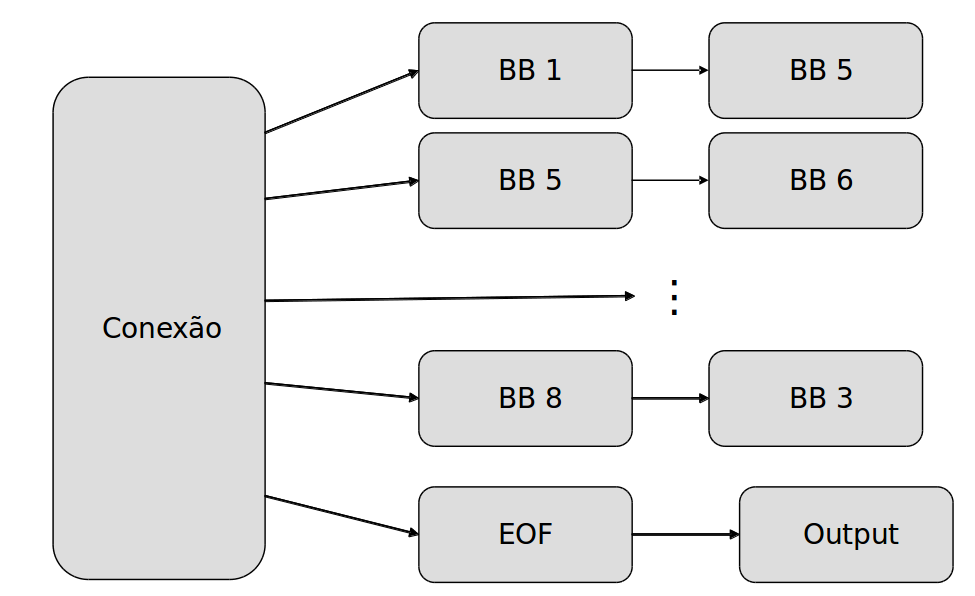
\includegraphics[width=\textwidth]{PyPolyBuilderGen}
\caption{Fluxograma ilustrativo do funcionamento do módulo \textit{general} do PyPolyBuilder.
A partir do arquivo de conexões fornecido pelo usuário, o PyPolyBuilder conecta os blocos de construção através dos átomos passados, também, pelo arquivo de conexão.
Ao chegar no final do arquivo, os arquivos de saída são gerados.}
\label{fig:PyPolyBuilderGen}
\end{figure}

Já no módulo geral, diferentemente do otimizado para dendrímeros, nenhuma geometria é pressuposta.
Por isso, ao invés de um único escalar para reger seu tamanho, um arquivo de conexões é necessário.
Nesse arquivo, a cada linha deve ser definido os índices de quais blocos devem se ligar e dos dois átomos que serão utilizados para a formação da ligação química.
O PyPolyBuilder lê essa lista enquanto cria a topologia e ao chegar no fim do arquivo, ele escreve a saída em arquivo.
O Fluxograma está ilustrado na Figura \ref{fig:PyPolyBuilderGen}.

Além do arquivo de conexões, as topologias de cada um dos blocos de construção utilizados devem ser fornecidas e, também, o arquivo contendo os parâmetros do campo de força.
Esse módulo foi satisfatoriamente utilizado para a geração de \textit{Hyper Branched Polymers} (HBP) propostos por Yu \textit{et al}\cite{Yu2016} em seu \textit{HBP Builder}.
Contudo, a abordagem do PyPolyBuilder é completamente determinística, diferentemente da geração estocástica do \textit{HBP Builder}.

\section{Propriedades}\label{Propriedades}

\subsection{Raio de giro}\label{RaioDeGiro}
O raio de giro médio quadrático nos fornece uma descrição quantitativa do tamanho de uma macromolécula.
Essa é uma propriedade amplamente conhecida e utilizada na ciência de polímeros e tem sido comumente utilizada, também, para a caracterização de dendrímeros. 
Para uma molécula com N átomos:

\begin{equation}
\langle R_g^2 \rangle  = \frac{1}{M} \Bigg \langle\sum_{i=1}^{N} [{m_i}(|\vec{r}_i-\vec{R}|^2)] \Bigg \rangle,
\end{equation}
onde, M é a massa total da molécula, $m_i$ é a massa do átomo i, $\textbf{r}_i$ o vetor de coordenadas do átomo i, $\textbf{R}$ é o vetor de coordenadas do centro de massa da molécula.

Foi feita uma análise avaliando a influência de se determinar o $R_g$ utilizando o centro de massa do bloco central ou do dendrímero como um todo. Como o principal objetivo deste trabalho é a validação do campo de força, foi decidido calcular o raio de giro com base no centro de massa do dendrímero completo já que essa é a forma mais comumente utilizada nos trabalhos encontrados na literatura.

\subsection{Asfericidade}\label{Fator de forma}\label{Asfericidade}
A forma dos dendrímeros é comumente avaliada com base nas razões de aspecto e no valor de asfericidade do mesmo, que dão uma ideia do quão esférico é a forma da molécula avaliada.

Para isso, obtemos os valores dos momentos de inércia (I) através do cálculo dos autovalores do tensor de forma ($\mat{G}$) e convencionando que $I_z > I_y > I_x$: \cite{Rapaport2005}

\begin{equation}
 \mat{G}_{mn} = \frac{1}{M} \sum_{i=1}^{N} [{m_i}(r_{mi}-{R_m})(r_{ni}-{R_n})]
\end{equation}
onde $m,n = x,y,z$, M é a massa total da molécula, $m_i$ é a massa do átomo i, $\textbf{r}_i$ o vetor de coordenadas do átomo i, $\textbf{R}$ é o vetor de coordenadas do centro de massa da molécula.

As razões de aspecto são frações envolvendo os momentos de inércia de diferentes eixos.
Essas relações mostram o quanto a projeção da molécula no plano envolvendo os eixos escolhidos divergem de um círculo, ou seja, quanto mais distante da unidade for a razão de aspecto, menos circular é a projeção da molécula naquele plano.
As razões de aspecto calculadas foram:

\begin{equation}
\frac{I_z}{I_y} \quad \text{e} \quad \frac{I_z}{I_x}
\end{equation}

Enquanto a asfericidade é obtida através da equação proposta por Rudnick e Gaspari\cite{rudnick1986}:

\begin{equation}
\delta = 1 - 3\frac{\langle I_2 \rangle}{\langle {I_1}^2 \rangle};
\end{equation}
onde $I_1 = I_x + I_y + I_z$ and $I_2 = {I_x}{I_y}+{I_x}{I_z}+{I_y}{I_z}$.

Nessa abordagem, quão mais esférica for a molécula, mais próximo de zero estará o valor de $\delta$.

\subsection{Funções de distribuição radial}\label{RDF}
As funções de distribuição radial (RDF) medem o número médio de átomos do tipo $\beta$ a uma distância r de átomos do tipo $\alpha$ dividido pelo número que um gás ideal de mesma densidade teria na mesma distância r.\cite{Allen2017}
Para que essa função seja avaliada computacionalmente, a distância r é discretizada em camadas de espessura $\Delta r$ e o número médio de átomos do tipo $\beta$ é contado dentro de cada esfera concêntrica ao redor dos átomos $\alpha$\cite{Allen2017}:

\begin{equation}
g_{\alpha\beta}(r) = (4\pi r^2\rho\Delta r)^{-1} \langle N_{\alpha\beta}(r; \Delta r) \rangle ,
\end{equation}
onde, $\rho$ é a densidade do meio, $\Delta r$ é a espessura considerada para a discretização do espaço e $\langle N_{\alpha \beta}(r;\Delta r) \rangle$ é o número médio de átomos do tipo $\beta$ dentro do intervalo $(r-\nicefrac{\Delta r}{2}, r+\nicefrac{\Delta r}{2})$ de um átomo do tipo $\alpha$.

Esses perfis radiais nos fornecem informação sobre como é a dispersão local de um grupo de átomos $\beta$ em relação à um grupo de átomos $\alpha$. 
As RDFs são também chamadas de perfis de densidade radial por avaliarem uma dendidade numérica relativa em relação à um meio ideal. Porém, não é raro encontrarmos curvas onde a função de distribuição radial não é normalizada pelo volume da casca esférica considerada. 
Esse tipo de análise é comum quando queremos o número absoluto de átomos do tipo $\beta$ dispersos ao redor de $\alpha$.
